%
% LaTeX template document for Leiden students
%
% vim: tw=80
%
%% The first piece of markup in an AASTeX v6.x document is the \documentclass
%% command. LaTeX will ignore any data that comes before this command. The 
%% documentclass can take an optional argument to modify the output style.
%% The command below calls the preprint style which will produce a tightly 
%% typeset, one-column, single-spaced document.  It is the default and thus
%% does not need to be explicitly stated.
%%
%%
%% using aastex version 6.3

\documentclass[a4,modern]{aastex63}

%% The default is a single spaced, 10 point font, single spaced article.
%% There are 5 other style options available via an optional argument. They
%% can be invoked like this:
%%
%% \documentclass[arguments]{aastex63}
%% 
%% where the layout options are:
%%
%%  twocolumn   : two text columns, 10 point font, single spaced article.
%%                This is the most compact and represent the final published
%%                derived PDF copy of the accepted manuscript from the publisher
%%  manuscript  : one text column, 12 point font, double spaced article.
%%  preprint    : one text column, 12 point font, single spaced article.  
%%  preprint2   : two text columns, 12 point font, single spaced article.
%%  modern      : a stylish, single text column, 12 point font, article with
%% 		  wider left and right margins. This uses the Daniel
%% 		  Foreman-Mackey and David Hogg design.
%%  RNAAS       : Preferred style for Research Notes which are by design 
%%                lacking an abstract and brief. DO NOT use \begin{abstract}
%%                and \end{abstract} with this style.
%%
%% Note that you can submit to the AAS Journals in any of these 6 styles.
%%
%% There are other optional arguments one can invoke to allow other stylistic
%% actions. The available options are:
%%
%%   astrosymb    : Loads Astrosymb font and define \astrocommands. 
%%   tighten      : Makes baselineskip slightly smaller, only works with 
%%                  the twocolumn substyle.
%%   times        : uses times font instead of the default
%%   linenumbers  : turn on lineno package.
%%   trackchanges : required to see the revision mark up and print its output
%%   longauthor   : Do not use the more compressed footnote style (default) for 
%%                  the author/collaboration/affiliations. Instead print all
%%                  affiliation information after each name. Creates a much 
%%                  longer author list but may be desirable for short 
%%                  author papers.
%% twocolappendix : make 2 column appendix.
%%   anonymous    : Do not show the authors, affiliations and acknowledgments 
%%                  for dual anonymous review.
%%
%% these can be used in any combination, e.g.
%%
%% \documentclass[twocolumn,linenumbers,trackchanges]{aastex63}
%%
%% AASTeX v6.* now includes \hyperref support. While we have built in specific
%% defaults into the classfile you can manually override them with the
%% \hypersetup command. For example,
%%
%% \hypersetup{linkcolor=red,citecolor=green,filecolor=cyan,urlcolor=magenta}
%%
%% will change the color of the internal links to red, the links to the
%% bibliography to green, the file links to cyan, and the external links to
%% magenta. Additional information on \hyperref options can be found here:
%% https://www.tug.org/applications/hyperref/manual.html#x1-40003
%%
%% Note that in v6.3 "bookmarks" has been changed to "true" in hyperref
%% to improve the accessibility of the compiled pdf file.
%%
%% If you want to create your own macros, you can do so
%% using \newcommand. Your macros should appear before
%% the \begin{document} command.
%%
%%
%% If you wish, you may supply running head information, although
%% this information may be modified by the editorial offices.
\shorttitle{Report Template}
\shortauthors{Kenworthy et al.}
%%
%% You can add a light gray and diagonal water-mark to the first page 
%% with this command:
%% \watermark{text}
%% where "text", e.g. DRAFT, is the text to appear.  If the text is 
%% long you can control the water-mark size with:
%% \setwatermarkfontsize{dimension}
%% where dimension is any recognized LaTeX dimension, e.g. pt, in, etc.
%%





% the color package allows us to define non-standard colours in the latex output
\usepackage{color}
\definecolor{darkblue}{rgb}{0.0, 0.0, 0.4}

% we use the hyperref package so that our links are clickable in a PDF reader
\usepackage{hyperref}
\hypersetup{colorlinks=true,citecolor=darkblue,linkcolor=black}

% tcolorbox allows a coloured box around text or math!
\usepackage{tcolorbox}






% the document begins here with the basic information first
\begin{document}

\title{Basic \LaTeX\ skills for Leiden Observatory Students}

% your name and address
\author[0000-0002-7064-8270]{M.A. Kenworthy}
\affil{Leiden Observatory, Leiden University, P.O. Box 9513, 2300 RA Leiden, The Netherlands}

\email{kenworthy@strw.leidenuniv.nl}

\date{April 2020}

% the abstract should be about one paragraph long and quicky summarise what the paper is describing
\begin{abstract}

We describe how to write a simple LaTeX document that students at Leiden Observatory can use to present their results.
%
These include how to format basic formulas, include graphics and how labelling and references are included in a document.

\end{abstract}

\section{Introduction}

\LaTeX\ is used by astronomers all over the world to produce scientific reports and to
prepare papers for submission to astronomical journals.
%
In this document we include a simple figure, some equations and some cross-referencing that shows
the power of \LaTeX.
%
It produces beautiful looking equations and is used by many physical science researchers across the world.
%
Taking time to learn \LaTeX\ now is a skill-set crucial for all astronomers.

\section{Making a \LaTeX\ document}

At the most basic, you write \LaTeX\ in a plain text file with an extension of \verb=.tex= - an example is the name of this document - \verb=leiden_report_template.tex=.
%
You can use any basic text editor to create and edit this text file.

You then run \verb=pdflatex= with this filename as an argument - 

\begin{verbatim}
pdflatex leiden_report_template.tex
\end{verbatim}

If your \LaTeX\ document contains references and labels within the document, you
may need to re-run the pdflatex command more than once.

\begin{verbatim}
pdflatex leiden_report_template.tex
pdflatex leiden_report_template.tex
\end{verbatim}

These commands then generate a PDF file that you can then read with your
favourite PDF viewer.

\section{Using aastex}


This document uses a \LaTeX\ package called AASTEX v6.3 to take the text and lay out the document in a specific way.
%
It is used by most of the big astronomy journals, so by writing your document and using this package, you are already most of the way to get it ready to submit it to a journal.
%
It is insalled on most of the STRW computers, so this should compile without a problem.


Both these packages are installed on the STRW computers and will automatically be found and included in your latex file.
%
If you are trying this on your laptop or another computer, it may not work.
%
You need to install both these packages.


\section{How to reference other Sections and Figures \label{mylabels}}

This sentence is in Section \ref{mylabels}.
%
If you read the tex file that produced this PDF, you will see that I did not refer to this Section by a number but with the latex command \verb=\ref{mylabels}=, and that in the Section header, you can see that there is a latex command \verb=\label{mylabels}=.
%
The \verb=\label= and \verb=\ref= are linked with a key, which is a piece of text which makes a unique label and marks a specific spot in the latex file.
%
In this case, the key is the word \verb=mylabels=.
%
Make sure you don't have duplicate keys in your latex file - all \verb=\label= commands should have unique key words in them.

In this way you can label figures, Sections, and Subsections in your latex document without worrying about keeping the numbering correct in your document.
%
\LaTeX\ does all of this calculation and bookkeeping for you, leaving you to write your report for your supervisor.

\section{How cite papers in your \LaTeX\ document}

The previous sections are all you need to know about writing and making a simple \LaTeX\ document.
%
The real power of \LaTeX\ comes with the way it handles citations.
%
Citations are when you make a statement in your paper which is based on someone
else's work.
%
You include a citation to that person's work, usually the surname of the first authour and the year it was published, e.g. Kenworthy et al. (2001).

Let's put in a reference from the file \verb=kenworthy.bib= : \citet{Quanz10b}

References are stored in another text file (here we use \verb=mybib.bib=) and
you then tell latex that there's a bibliography file by using the command
\verb=\bibliography{mybib}=.
%
If you look at the \verb=tex= file for this document, though, you'll see that there is another command:

\begin{verbatim}
\bibliographystyle{aasjournal}
\bibliography{kenworthy}
\end{verbatim}

The first command, \verb=\bibliographystyle{nsf}= tells \LaTeX\ to look for a file called \verb=nsf.bst= in the current directory - this file tells \LaTeX\ how to make the references look in the final document.

To build a \LaTeX document with a bibliography included in it, you need to run four commands in this sequence:

\begin{verbatim}
pdflatex test
bibtex test
pdflatex test
pdflatex test
\end{verbatim}

The program \verb=bibtex= does the work of pulling out your references and making them look correct for insertion into your output document.

There are several styles of citing other people's work:

In \citet{Wagner20} there is an image of the disk PDS~201 taken using an APP coronagraph, similar to the one used successfully before \citep{Quanz10}.
%
When you have several papers \citep{Quanz10b,Kenworthy20} you can also chain them at the end too \citet{2019ApJS..244...15M,Quanz10}, and even if you have two references with the same name and year, bibtex works that out for you \citep{Quanz10,Quanz10b}.

You can also put words and phrases within the citation \citep[e.g.][ as an example]{Kenworthy20} - just read the tex file and see how you can do this.


\begin{figure}[htp]
\centering
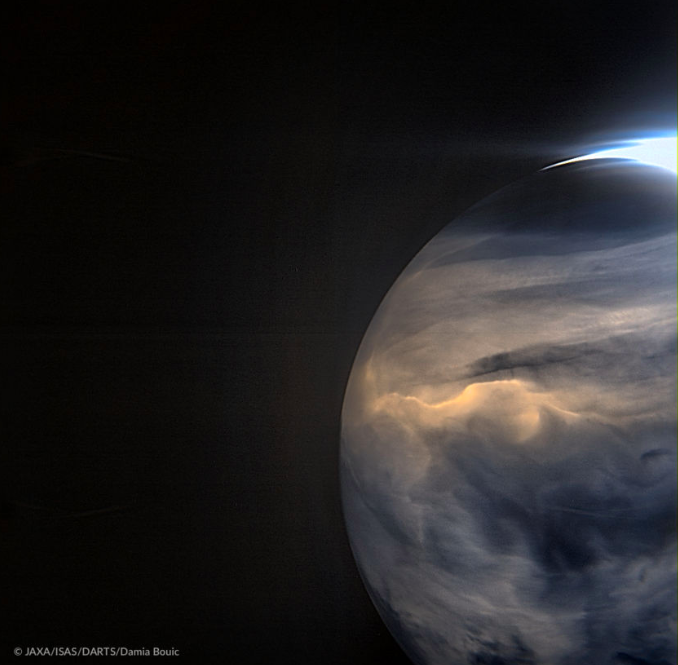
\includegraphics[angle=0,width=1.0\textwidth]{venus_ir}
\caption{Venus captured by the Japanese Akatsuki spacecraft's IR2 camera, processed by Damia Bouic, as seen at this \href{https://twitter.com/CosmicRami/status/1253293199897944066}{Tweet}}
\end{figure}


\section{Using ADS to build your own bibtex file}

The Astrophysics Data Service is one of the most useful web sites for research astronomers.
%
The ADS allows you to search for astronomy papers, download and read them, and you can export the BibTeX for a citation of all the papers you find.
%
You can then copy these citations into your bibtex file, and use this file for the rest of your career without having to type in the citation manually.

Going to the search page of the ADS, you can search by author, first author, year, or many other search terms. Searching on Kenworthy gives the resultant page in Figure~\ref{01find}.
%
You can select one or more papers by clicking the blue checkboxes on the left of the paper title, and then go to the right hand side, check on 'export' and a drop down menu will appear (see Figure~\ref{02}), and then go to BibTeX.
%
You are then shown a grey window with the text that contains the bibtex references. You can either select the text manually with your cursor, or use the ``Copy to Clipboard'' button.

Open your bibtex file and post the text in.

I would strongly suggest changing the bibtex key to something other than the alphanumeric code, and I suggest ``Last name+Last two digits of the publishing year'', e.g. Kenworthy19, Miller13, Markov98.

If you have one first author with two publications in the same year, label the second reference you add with an extra letter, so: Kenworthy15, Kenworthy15b, Kenworthy15c.

It is IMPORTANT that you do not change the key once you've started using the citations in your documents. You may be tempted to order the a,b,c.... references in month order, but do not do that, since your old latex documents will then have the incorrect references.

\begin{figure}[htp]
\centering
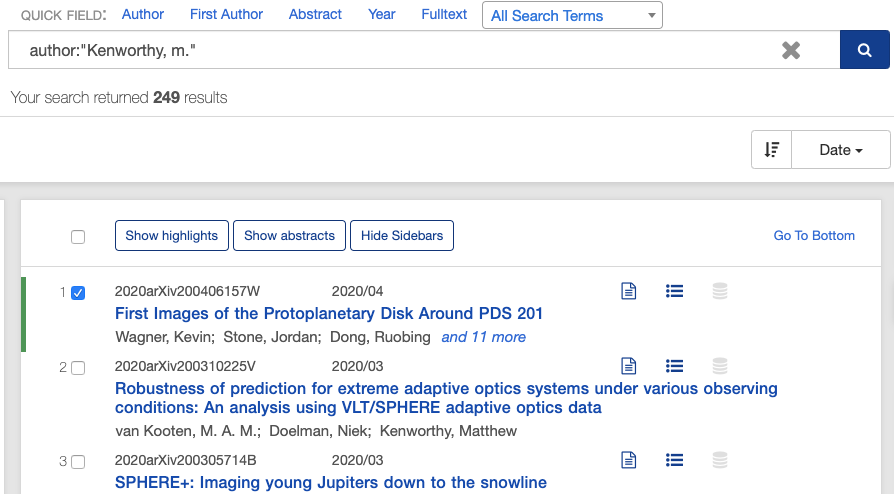
\includegraphics[angle=0,width=0.6\textwidth]{01_find_ref}
\caption{ \label{01find}Results from the search showing one paper selected with the blue check box.}
\end{figure}


\begin{figure}[htp]
\centering
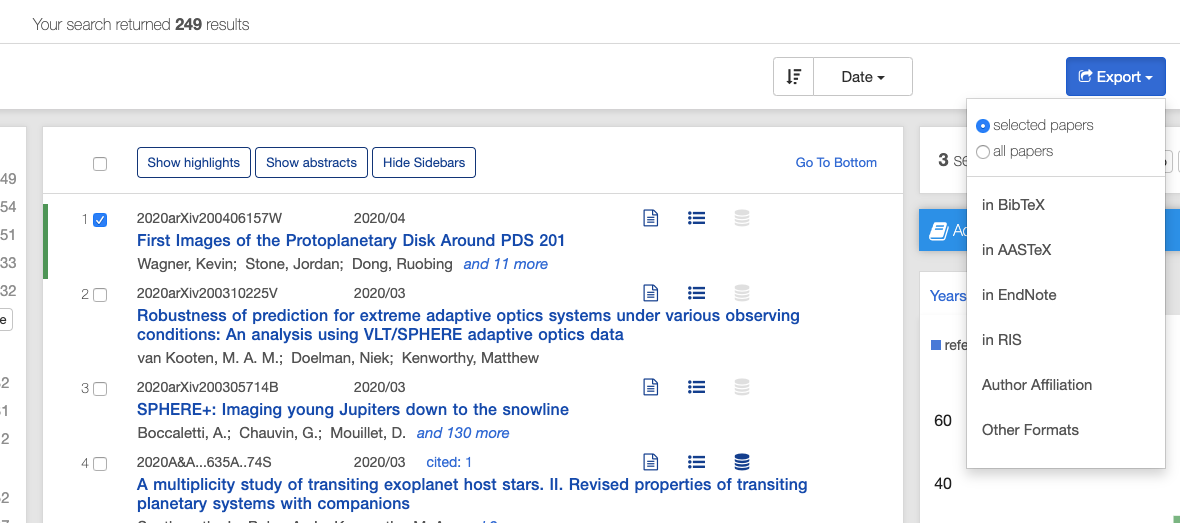
\includegraphics[angle=0,width=0.6\textwidth]{02_select_export_citations}
\caption{ \label{02}The drop down menu under ``Export'' and going down to BibTeX and selecting it.}
\end{figure}


\begin{figure}[htp]
\centering
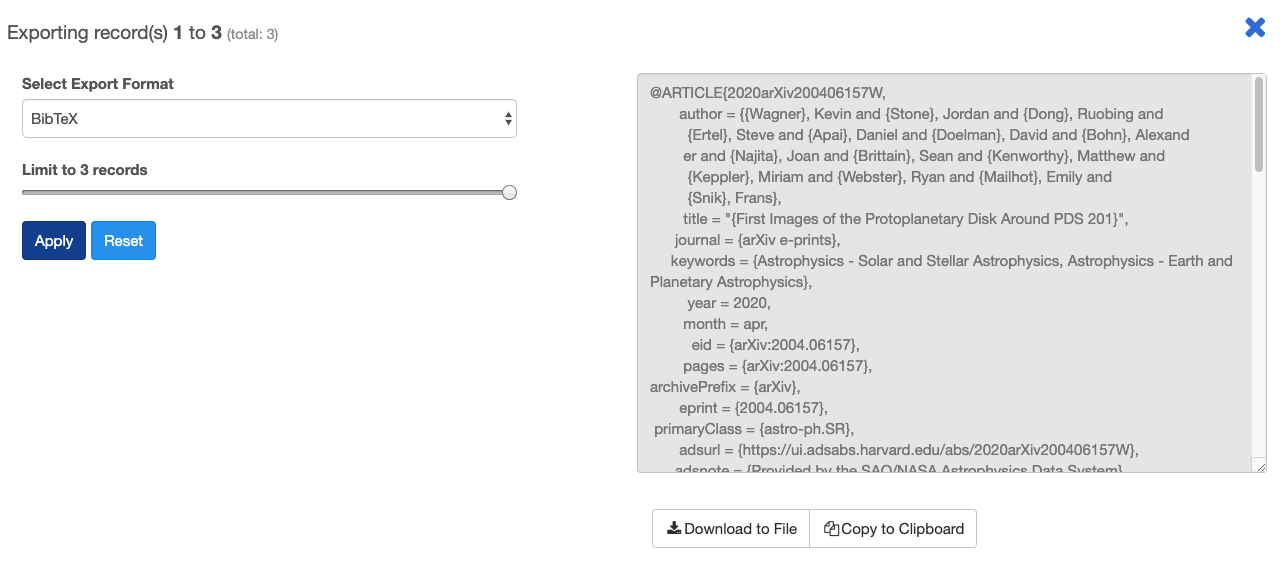
\includegraphics[angle=0,width=0.6\textwidth]{03_cut_and_paste}
\caption{ \label{03bib}Selecting the option produced the BibTeX output in the grey window on the right. This can be cut and pasted manually or using the ``Copy to Clipboard'' button.}
\end{figure}


\begin{figure}[htp]
\centering
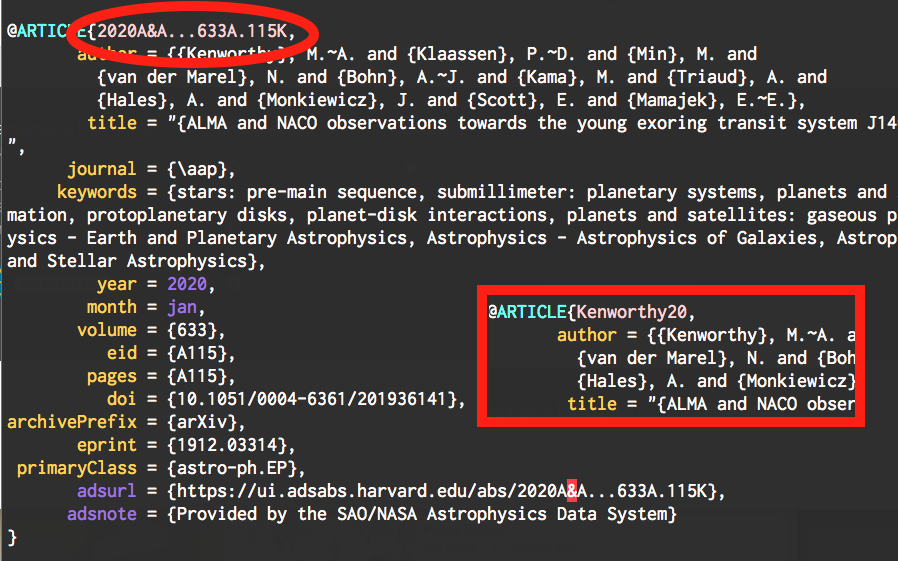
\includegraphics[angle=0,width=0.6\textwidth]{04_key}
\caption{ \label{04keyrename} (optional step) Rename the bibcode key to something more familiar - in this example, the first author's surname followed by the last two numbers of the year of publication.}
\end{figure}

\begin{tcolorbox}[colback=red!5!white,colframe=red!75!black,title=CAUTION]

This is outdated material, kept here for reference

\end{tcolorbox}

\section{Figures don't look well centred in the document}


Postscript figures generated by several graphics programs seem to work with the usual compilation route for \LaTeX, but seem to fail with \verb=pdflatex=.
%
Encapsulated postscript files have a BoundingBox defined in their header which is used by pdflatex to generate the right PDF image.
%
So, we need a two step process - convert the postscript file into an encapsulated postscript file, and the convert the encapsulated postscript file into a PDF file.

Step 1:

Starting with a Posctscript file called \verb=your_figure.ps= and run this \verb=ps2eps= command on it:

\begin{verbatim}
ps2eps -B -l -g -f your_figure.ps
\end{verbatim}

This will produce a file called \verb=your_figure.eps= which is an Encapsulated Postscript version of \verb=your_figure.ps=.

The command line flags are: \verb=-f= to force overwrite of any old BoundingBox defined in the figure, \verb=-B= ignores the current Bounding Box, \verb=-g= uses the ghostscript Bounding Box device instead of the externally called Bounding Box routine, and \verb=-l= expands all the Bounding Box dimensions by one point in size so that there is a thin white line of speace around the figure.

Step 2:

Use the \verb=ps2pdf= routing to take \verb=your_figure.eps= and produce
\verb=your_figure.pdf=.

\begin{verbatim}
ps2pdf -dEPSCrop your_figure.eps
\end{verbatim}

The \verb=EPSCrop= option tells \verb=ps2pdf= to use the BoundingBox defined in the eps figure.

\section{Conclusions}

This is a simple \LaTeX\ document that shows how you can include figures with captions and not worry about the bookkeeping involved in correctly numbering the figures and sections.

\bibliographystyle{aasjournal}
\bibliography{kenworthy}

\end{document}

